\documentclass[a4paper,11pt]{article}
\usepackage[utf8]{inputenc}
\usepackage[frenchb]{babel}
\usepackage{amssymb}
\usepackage{amsmath}
\usepackage{amsthm}
\usepackage{mathrsfs}
\usepackage{array}
\usepackage{graphicx}
\usepackage[usenames,dvipsnames]{color}
\usepackage{listings}
\usepackage{arydshln}
\usepackage{slashbox}
\usepackage{subfigure}
\usepackage{pdflscape}
\usepackage{multirow}
%\usepackage{cancel}
%\usepackage[bookmarks = false]{hyperref}
\usepackage{enumitem}
\usepackage[left=1.75cm, right=1.75cm, top=2cm, bottom=2cm]{geometry}

\newcommand{\ttsee}[1]{Voir \texttt{#1}\paragraph{}}
\newcommand{\ttseek}[1]{Voir package \texttt{#1}\paragraph{}}


% Initialisation de listings
%\definecolor{mymauve}{rgb}{0.63,0.13,0.94}
%\definecolor{mygreen}{rgb}{0.13,0.55,0.13}
%\definecolor{mybeige}{rgb}{0.99,0.99,0.86}
\definecolor{bcg}{rgb}{0.95,0.95,0.95}
\definecolor{light-gray}{gray}{0.50}
\lstset{
	backgroundcolor=\color{bcg},   % choose the background color; you must add \usepackage{color} or \usepackage{xcolor}
    columns=flexible,
	%numbers = left,				    % placement de la numérotation des lignes
	numberstyle = \small,        	% taille du numéro de ligne
	stepnumber = 1,              	% ???
	numbersep = 10pt,            	% taille de l'espace de séparation entre numéro de ligne et code
	showspaces = false,          	% montrer les espaces
	showstringspaces=false,         % enlever les espaces str
	showtabs = false,            	% montrer les tabulations
	tab = rightarrowfill,        	% ???
	tabsize=2,						% tabulation size
	language = Java,             	% langage utilisé
	basicstyle = \footnotesize\tt,	% ???
	captionpos = b,					% ???
	linewidth=\linewidth,			% largeur de la fenetre de code
	breaklines = true,				% ???
	commentstyle = \color{light-gray}, % définition de la couleur des commentaires
	%stringstyle = \color{mymauve},  % définition de la couleur des chaines de caractères
	%identifierstyle = \ttfamily,    % ???
	keywordstyle = \color{blue},	% définition de la couleur des mots clés
	%frame=single,
	%backgroundcolor=\color{mybeige},
	extendedchars=true				% étend les caractères pouvant être utilisés
}
\setlist[itemize,1]{label=$\bullet$}
%\author{Mormont Romain}
%\title{Synthèse : Base de données (Pierre Wolper)}
%\date{Année académique 2013-2014}

\begin{document}
\thispagestyle{empty}
\rule{1\linewidth}{1px}
{ \sc
\begin{center}
{\small University of Liège}\\
{\small Faculty of Applied Sciences}

\end{center}

\vfill
\begin{center}

{\Huge Sushi++ compiler\\}
\end{center}
\begin{center}
{\Huge Project report  {\LARGE \tt [INFO2049]} }
\end{center}
\begin{center}
\textbf{Magera Floriane}\\
{\small 1$^{\text{st}}$ master in computer engineering}\\
{\small Option : Computer systems and networks}\\
{\small s111295} \\ 
\textbf{Servais Fabrice}\\
{\small 1$^{\text{st}}$ master in computer engineering}\\
{\small Option : Computer systems and networks}\\
{\small s111093} \\ 
\textbf{Mormont Romain}\\
{\small 1$^{\text{st}}$ master in computer engineering}\\
{\small Option : Intelligent systems}\\
{\small s110940} \\ 
\end{center}

\vfill
\begin{center}
Academic year 2014-2015\\
\end{center}
}
\rule{1\linewidth}{1px}
\newpage
\thispagestyle{empty}
\tableofcontents
\newpage
\setcounter{page}{1}
\section{Introduction}
In the context of the course INFO0085, we had to develop a compiler for a handmade programming language called \textbf{Sushi++}. This language is garbage-collected and halfway between a functional and an imperative language of which the keywords are inspired from the \textit{sushi food} lexical field. The first part of the report describes both syntax and semantic of the language (section \ref{sec:language}) and the second details the compiler organization and algorithms (section \ref{sec:compiler}). The Section \ref{sec:runtime} presents the organization of the small runtime library handling the garbage collector. Finally, in the Section \ref{sec:improv}, the improvements that could be made are discussed. 
\section{Language}
\label{sec:language}
\subsection{General information}
\subsection{Type system}
\label{ssec:types_s}
The \textit{Sushi++} language is a strongly and statically typed language. Nevertheless, to alleviate the programmer's work, the type system is made as unobtrusive as possible and types are inferred during compilation. The only presence of types in the language is the \textit{function parameters hinting} mechanism : the parameter type can be specified next to the parameter name in the a function declaration (see Section \ref{sssec:decl_func}). The available types are :

\begin{itemize}
	\item \texttt{bool} : \textit{true} or \textit{false}
	\item \texttt{char} : a character
	\item \texttt{int} : an integer $\in [-2147483648, 2147483647]$
	\item \texttt{float} : a single-precision floating point value $\in [-3.403 \times 10^{38},  3.403 \times 10^{38}] $
	\item \texttt{array} : an array of elements (see Section \ref{sssec:arrays})
	\item \texttt{list} : a list of elements (see Section \ref{sssec:lists})
	\item \texttt{string} : a string
	\item \texttt{function} : a function 
	\item \texttt{void} : return type for function that doesn't return anything
\end{itemize}
\subsubsection{Arrays}
\label{sssec:arrays}
\paragraph{Idea}
The \texttt{array} type represents a sequence of elements having a given type \textit{T} and that are stored sequentially in the memory. This structure has the same behaviour as a vector data structure in terms of complexity. The \textit{Sushi++} arrays cannot stored any type of data, \textit{T} can only be one among : \texttt{int}, \texttt{float}, \texttt{char}, \texttt{string}, \texttt{bool}. The index of an array is an integer in the interval $[0, \text{array size}]$. Arrays are passed to function and returned by reference (they are never copied).
\paragraph{Syntax}
To construct an array, its elements must be listed between the array delimiters \texttt{\#[} and \texttt{]\#} and separated by commas  : 
\begin{itemize}
	\item array of integers : \texttt{\#[ 1, 2, 3, 4 ]\#} 
	\item array of strings : \texttt{\#[ "str1", "str2", "str3", "str4" ]\#} 
	\item assigning a variable : \texttt{maki a = \#[ true, false ]\#}
\end{itemize}
To access an element in the array, the C-like array-access operator \texttt{[]} can be used with a valid index. 
\begin{center}
	\texttt{maki first\_element = array[0]}
\end{center}
A set of built-in functions are provided to the programmer to handle arrays. They are listed as follows in a C-like format :
\begin{itemize}
	\item \texttt{int array\_size\_T(array A)} : return the size of the array
	\item \texttt{void array\_clear\_T(array A)} : empty the array
	\item \texttt{void array\_push\_T(array A, T element)} : push an element at the last position of the array
	\item \texttt{T array\_pop\_T(array A)} : pop the element at the last position of the array
	\item \texttt{T array\_get\_T(array A, int i)} : return the element at the position \texttt{i} of the array
	\item \texttt{void array\_set\_T(array A, int i, T element)} : replace the element at the position \texttt{i} by \texttt{element}
	\item \texttt{void array\_insert\_T(array A, int i, T element)} : insert \texttt{element} at the position \texttt{i}
\end{itemize}
\paragraph{Memory} Arrays are \textbf{heap-allocated} and their memory is managed at runtime with a garbage collector (see Section \ref{ssec:garabage_collector}).

\subsubsection{Lists} 
\label{sssec:lists}
The construction of lists follows the same principles as the construction of array except that the delimiters are the curly brackets characters : 
\begin{itemize}
	\item array of integers : \texttt{\{ 1, 2, 3, 4 \}} 
	\item array of strings : \texttt{\{ "str1", "str2", "str3", "str4" \}} 
	\item assigning a variable : \texttt{maki a = \{ true, false \}}
\end{itemize}
Lists \textit{cannot} be accessed with the array-access operator. Nevertheless, a set of built-in functions are provided for interacting with them (inspired from standard C++ lists interface):
\begin{itemize}
	\item \texttt{int list\_size(List l)} : return the size of the list 
	\item \texttt{bool list\_empty(List l)} : return true if the list is empty, false otherwise
	\item \texttt{void list\_clear(List l)} : clear the content of the list
	\item \texttt{T list\_front\_T(List l)} : return the element at the front of the list
	\item \texttt{T list\_back\_T(List l)} : return the element at the back of the list
	\item \texttt{T list\_pop\_front\_T(List l)} : remove and return the element at the front of the list 
	\item \texttt{T list\_pop\_back\_T(List l)} : remove and return the element at the back of the list
	\item \texttt{void list\_push\_front\_T(List l)} : push an element at the front of the list
	\item \texttt{void list\_push\_back\_T(List l)} : push an element at the back of the list
	\item \texttt{T list\_get\_T(List l, int pos)} : get the element at the given position of the list
	\item \texttt{void list\_insert\_T(List l, int pos, T elem)} : insert an element at the given position of the list
	\item \texttt{T list\_remove\_T(List l, int pos)} : remover the element at the given position of the list
\end{itemize}
\paragraph{Memory} Lists are \textbf{heap-allocated} and their memory is managed at runtime with a garbage collector (see Section \ref{ssec:garabage_collector}).

\subsection{Declarations}

The \textit{Sushi++} language provides declaration syntax for both functions and variables. The declaration keyword \texttt{maki} is common to both declaration. The declared structured can be used using an identifier. The \textit{Sushi++} identifiers must match the following regular expression "\texttt{{[a-zA-Z]}({[-0-9A-Za-z\_]}*{[0-9A-Za-z\_]})*}".
\subsubsection{Functions}
\label{sssec:decl_func}
\paragraph{Idea} The function declared with the \texttt{maki} keyword are called \textbf{named function} in opposition to anonymous function (or \textit{soy functions}, see Section \ref{sssec:soy_func}). As soon as it is declared, a function can be either called (see Section \ref{sssec:func_call}) or used as expression (passed as parameter). A declared named function is accessible in the scope in which it is declared and its nested scopes (including the function own scope).
\paragraph{Syntax}  The named function declaration syntax is the following : 
\begin{center}
\texttt{maki} \textit{function\_name} \{\textit{parameter\_name}[\texttt{<} \textit{type} \texttt{>}]\} \texttt{:} \textit{function\_body} \texttt{;;}
\end{center}
The \textit{type} element must be one of the types listed in the Section \ref{ssec:types_s} except \texttt{void}.
\subsubsection{Variables}
\paragraph{Idea} A variable must be assigned a value when it is declared. It is accessible in the scope in which it is declared and its nested scopes but \textbf{cannot be captured} in a function. A variable can only by reassigned a value having the same type as the one initially assigned.
\paragraph{Syntax} Several variables can be declared with a single \texttt{maki}, the different declarations must be separated by commas : 
\begin{center}
\texttt{maki} \textit{variable\_name} = expression \{, \textit{variable\_name} = expression \}
\end{center}
\subsection{Expressions}
\subsubsection{Soy functions}
\paragraph{Idea} Soy functions or anonymous functions are functions that are not bound to an identifier. They can either be used as value (passed as parameters), be called (see Section \ref{sssec:func_call}) or stored into a variable.
\paragraph{Syntax} A soy function is declared by using the \texttt{soy} keyword : 
\begin{center}
	\texttt{(soy} \{\textit{parameter}[\texttt{<}\textit{type}\texttt{>}]\} \texttt{:} \textit{function\_body} \texttt{)}
\end{center}
Various usages :
\begin{itemize}
	\item Storing an anonymous function in a variable : \texttt{ maki f = (soy x : nori x) }
	\item Passing an anonymous function as parameter : \texttt{ call func (soy x : nori x) a }
	\item Calling an anonymous function : \texttt{ call (soy x : nori x) 1 }
\end{itemize}
\label{sssec:soy_func}
\subsubsection{Function calls}
\label{sssec:func_call}
\paragraph{Idea} A function call is triggered with the \texttt{call} keyword followed by a function name or an expression that can be evaluated as a function.  The keyword \texttt{call} is meant to prevent the ambiguity between a function call and a variable utilisation. A function call must be braced when its arguments are placed on several lines or if it is embedded into another expression.
\paragraph{Syntax} The syntax for calling a function is the following :
\begin{center}
	\texttt{call} (\textit{function\_name}$|$soy\_expression) \{ argument \}
\end{center}
Various usages :
\begin{itemize}
	\item Calling a function : \texttt{ call func param1 param2 }
	\item Calling an anonymous function : \texttt{ call (soy x : nori x) 1 }
	\item Embedded call : \texttt{a = (call func c d) }
\end{itemize}
\subsubsection{Operators}
The \textit{Sushi++} language provides a set of operators for expressing operations on flat types. These operators are listed in the Table \ref{tab:operators} which describes their properties. The precedence and associativity was inspired from the C language. Therefore, in general, operators are left associative except for the assignment\footnote{so that they can be chained} and exponentiation. The precedence number given in the table decreases with the priority of the operator.
\begin{table}
	\center
	\footnotesize
	\begin{tabular}{|c|c|c|c|p{0.30\linewidth}|cc|}
	\hline
	\multirow{2}{*}{\textbf{Op.}} & \multirow{2}{*}{\textbf{Arity}} & \multirow{2}{*}{\textbf{Assoc.}} & \multirow{2}{*}{\textbf{Prec.}} & \multirow{2}{*}{\textbf{Comment}} & \multicolumn{2}{c|}{\textbf{Operand types}} \\
	 & & & & & Operand 1 & Operand 2 \\
	\hline
	\texttt{op ++} & 1 & / & 1 & Postfix increment & \multicolumn{2}{c|}{$\{\texttt{int}, \texttt{float}\}$}\\
	\texttt{op --} & 1 & / & 1 & Postfix decrement & \multicolumn{2}{c|}{$\{\texttt{int}, \texttt{float}\}$}\\
	\texttt{++ op} & 1 & / & 2 & Prefix increment & \multicolumn{2}{c|}{$\{\texttt{int}, \texttt{float}\}$}\\
	\texttt{-- op} & 1 & / & 2 & Prefix decrement & \multicolumn{2}{c|}{$\{\texttt{int}, \texttt{float}\}$}\\
	\texttt{op1 ** op2} & 2 & right & 3 & Exponent & $\{\texttt{int}, \texttt{float}\}$ & \texttt{int} \\
	\texttt{op1 . op2} & 2 & right & 3 & String concatenation & \texttt{string} & \texttt{string} \\
	\texttt{- op} & 1 & / & 4 & Unary minus & \multicolumn{2}{c|}{$\{\texttt{int}, \texttt{float}\}$}\\
	\texttt{\~{} op} & 1 & / & 5 & Bitwise not & \multicolumn{2}{c|}{\texttt{int}}\\
	\texttt{! op} & 1 & / & 5 & Logical not & \multicolumn{2}{c|}{\texttt{bool}}\\
	\texttt{op1 * op2} & 2 & left & 6 & Mutliplication & $\{\texttt{int}, \texttt{float}\}$ & same as \texttt{op1}\\
	\texttt{op1 / op2} & 2 & left & 6 & Division  & $\{\texttt{int}, \texttt{float}\}$ & same as \texttt{op1}\\
	\texttt{op1 \% op2} & 2 & left & 6 & Modulo & \texttt{int} & \texttt{int} \\
	\texttt{op1 + op2} & 2 & left & 7 & Addition  & $\{\texttt{int}, \texttt{float}\}$ & same as \texttt{op1}\\
	\texttt{op1 - op2} & 2 & left & 7 & Substraction & $\{\texttt{int}, \texttt{float}\}$ & same as \texttt{op1}\\
	\texttt{op1 >> op2} & 2 & left & 8 & Right shift & \texttt{int} & \texttt{int} \\
	\texttt{op1 << op2} & 2 & left & 8 & Left shift & \texttt{int} & \texttt{int} \\
	\texttt{op1 < op2} & 2 & left & 9 & Greater than & $\{\texttt{int}, \texttt{float}\}$ & same as \texttt{op1}\\
	\texttt{op1 > op2} & 2 & left & 9 & Equal to & $\{\texttt{int}, \texttt{float}\}$ & same as \texttt{op1}\\
	\texttt{op1 <= op2} & 2 & left & 9 & Less or equal to & $\{\texttt{int}, \texttt{float}\}$ & same as \texttt{op1}\\
	\texttt{op1 >= op2} & 2 & left & 9 & Greater or equal to & $\{\texttt{int}, \texttt{float}\}$ & same as \texttt{op1}\\
	\texttt{op1 != op2} & 2 & left & 10 & Not equal to & $\{\texttt{int}, \texttt{float}, \texttt{bool}\}$ & same as \texttt{op1}\\
	\texttt{op1 == op2} & 2 & left & 10 & Equal to & $\{\texttt{int}, \texttt{float}, \texttt{bool}\}$ & same as \texttt{op1}\\
	\texttt{op1 \& op2} & 2 & left & 11 & Bitwise and & \texttt{int} & \texttt{int} \\
	\texttt{op1 \^{} op2} & 2 & left & 12 & Bitwise xor & \texttt{int} & \texttt{int} \\
	\texttt{op1 | op2} & 2 & left & 13 & Bitwise or & \texttt{int} & \texttt{int} \\
	\texttt{op1 \&\& op2} & 2 & left & 14 & Logical and & \texttt{bool} & \texttt{bool} \\
	\texttt{op1 || op2} & 2 & left & 15 & Logical or & \texttt{bool} & \texttt{bool} \\
	\texttt{op1 += op2} & 2 & right & 16 & Addition assignment  & $\{\texttt{int}, \texttt{float}\}$ & same as \texttt{op1}\\
	\texttt{op1 -= op2} & 2 & right & 16 & Substraction assignment & $\{\texttt{int}, \texttt{float}\}$ & same as \texttt{op1}\\
	\texttt{op1 *= op2} & 2 & right & 16 & Mutliplication assignment & $\{\texttt{int}, \texttt{float}\}$ & same as \texttt{op1}\\
	\texttt{op1 /= op2} & 2 & right & 16 & Division assignment  & $\{\texttt{int}, \texttt{float}\}$ & same as \texttt{op1}\\
	\texttt{op1 \%= op2} & 2 & right & 16 & Modulo assignment & \texttt{int} & \texttt{int} \\
	\texttt{op1 **= op2} & 2 & right & 16 & Exponent assignment & $\{\texttt{int}, \texttt{float}\}$ & \texttt{int} \\
	\texttt{op1 .= op2} & 2 & right & 16 & Concatenation assignment & \texttt{string} & \texttt{string} \\
	\hline
	\end{tabular}
	\caption{Sushi++ operators}
	\label{tab:operators}
\end{table}
\subsection{Statements}
\subsubsection{Loops}
The \textit{Sushi++} language provides three kinds of loop. 
\paragraph{Condition-controlled loop} This loop is called \texttt{roll} and behaves like a C while loop. The scope containing this code fragment is delimited by the end of line following the condition and the scope delimiter \texttt{;;}. The condition must be an expression of type \texttt{bool}, otherwise the compiler will return a type error. . The syntax is the following :
\begin{center}
	\begin{minipage}{0.20\linewidth}
		\texttt{roll} \textit{condition} \\
		\text{ }\text{ }\text{ }\text{ }\textit{roll scope}\\
		\texttt{;;}\\
	\end{minipage}
\end{center}
\paragraph{Counter-controlled loop} This loop is called \texttt{for} and behaves like a C for loop. Again, the condition must be an expression of type \texttt{bool}. Moreover, the initializer and update part must contain a modifying expressions (assignment or increment). The syntax is the following :
\begin{center}
	\begin{minipage}{0.50\linewidth}
		\texttt{for} \textit{init expression}\texttt{, }\textit{condition}\texttt{, }\textit{update expression} \\
		\text{ }\text{ }\text{ }\text{ }\textit{for scope}\\
		\texttt{;;}\\
	\end{minipage}
\end{center}
\paragraph{Collection-controlled loop} This loop is called \texttt{foreach} and is made for iterating over lists. At the first iteration, the element at the front of the list is stored in the iteration variable. Then, at each iteration, the same goes for next value till the list was completely covered. The syntax is the following :
\begin{center}
	\begin{minipage}{0.35\linewidth}
		\texttt{foreach} \textit{list expression} \texttt{as} \textit{variable} \\
				\text{ }\text{ }\text{ }\text{ }\textit{foreach scope}\\
		\texttt{;;}\\
	\end{minipage}
\end{center}
\subsubsection{Conditionals}
\subsubsection{Switch}
\section{Compiler}
\label{sec:compiler}
\subsection{General information}
The \textit{Sushi++} compiler is implemented in standard C++ (version c++11). It is organized around the \texttt{SppCompiler} class which coordinates the various phases. The execution of the compiler can be tuned with various parameters (verbosity, optimization, input file path, output file path,...). The parameters parsing and analysis is encapsulated into the \texttt{CompilerSettings} object which provides a set of functions for knowing the values of the parameters. \\
The compiler follows the classical architecture :
\begin{itemize}
	\item Lexical and syntax analysis
	\item Semantic analysis
	\item Intermediate code generation
	\item Optimization and executable generation
\end{itemize}
The first phase uses \texttt{flex} and \texttt{bison} to generate an abstract syntax tree as an \texttt{ast::AbstractSyntaxTree} object. The tree nodes  classes are defined in the folder \texttt{ast/nodes} and are all subclasses of the \texttt{ast::ASTNode} class. While the base class implements a generic tree structure by storing pointers to parent and children nodes, the derived classes contains accessors to children defining the actual abstract syntax tree structure. To perform operations on the tree during the second and third phases, the visitor pattern was implemented. The visitors base class is \texttt{visitor::ASTVisitor} in the folder \texttt{ast/visitor} and every pass on the tree is implemented in its own visitor class :
\begin{enumerate}
	\item Function table populating and termination checking (\texttt{visitor::FunctionTableVisitor})
	\item Variable table populating (\texttt{visitor::VariableTableVisitor})
	\item Type inference (\texttt{visitor::TypeInferenceVisitor})
	\item Code generation (\texttt{visitor::CodeGenVisitor})
\end{enumerate}
As the initial visitor class (\texttt{visitor::PrintASTVisitor}) was designed parameter-free and that refactoring it would have taken too much time. Passing parameters is handled with the \texttt{visitor::VisitorParameters} class.  \\ 
The errors formatting and storing is encapsulated by the class \texttt{ErrorHandler} to which are passed the various errors generated during a phase.
\subsection{Lexical and syntax analysis}
\label{ssec:lex_synt}
At the beginning of the project, the choice was made to use \texttt{bison} and \texttt{flex} (versions \texttt{3.0.2} and \texttt{2.5.35} respectively) for the syntax and lexical analysis phases. This was motivated by the fact that many projects (including the integrated project) were ongoing during the development of this part of the compiler. So we decided to use existing tools to reduce the workload so that we could deliver a function syntax and lexical analysis for the first deadline. Among the existing tools, we have decided to use \texttt{bison} and \texttt{flex} because our compiler is developed in C++ and that integration would be easier.
\\ \\
The parser is implemented in the bison file \texttt{parser/spp\_parser.y} and the lexer in \texttt{scanner/spp\_scanner.lex}. Here are the elements that are worth to be mentioned :
\begin{itemize}
	\item the tree is built bottom up (as bison implements a bottom-up parser). Every time a rule is matched, the corresponding node is allocated and constructed. At construction, both its children and some location information (as \texttt{ast::NodeLocation} objects) are given to the node through the constructor.
	\item at the starting rule of the grammar, the abstract syntax tree object is allocated, his root is set with the node at the top of the built tree and is given to the \texttt{SppCompiler} object.
	\item adding errors to the error handler is done in the \texttt{yyerror} error function so that the built-in error reporting of bison can be used
	\item the operator precedence and associativity are handled with the dedicated bison constructs (see Table \ref{tab:operators})
	\item the semantic type of the nodes is unfortunately \texttt{void*} (see Section \ref{ssec:flaws_syntax})
	\item as the grammar is accepted by bison without conflicts \textbf{it is} LALR(1) and therefore \textbf{LR(1)}
	\item in the lexer file, a catch-all rule was added to generate the lexical errors when an unknown sequence is found
\end{itemize}
\subsection{Semantic analysis}
\subsubsection{Scope checking}
In order to perform scope checking, we implemented two visitors. The first one aim's is mainly to discover function's declarations and is named \texttt{FunctionTableVisitor}, while the second one \texttt{SymbolTableVisitor} will be the one to detect most semantic errors. The two visitors visit the abstract syntax tree and fill in the two symbol tables we maintain. There is one for the functions and one for the variables. The first one is filled by the first visitor and the second one by the second visitor. A little flaw is that the symbol table destined for variables may contain functions too. Sometimes we can only distinguish between a variable and a function at the inference step (in the case of an function passed as an argument for example).
\paragraph{The \texttt{FunctionTableVisitor}} is also used for termination checking, as will be explained in the next paragraph. There was a need to visit two times the tree because a function may be called before its definition. So at this level, the visitor adds informations about the functions defined in the code in the part of the symbol table corresponding to the scope containing the function's declaration. The information yielded is the name, the location and the argument's name of the function. Note that the arguments are also added in the variable symbol table in the scope corresponding to the function body.

\paragraph{The \texttt{SymbolTableVisitor}} fills the variable symbol table and checks that each variable was well declared and that each function call corresponds to a function repertoried by the \texttt{FunctionTableVisitor}. We decided to forbid closures.  
\subsubsection{Termination checking}
The termination checking is implemented in the \texttt{FunctionTableVisitor}. We made it as simple and light as possible : we implemented it with booleans. In our language, all the instructions that may contain a return are represented by the non-terminal token Statement. Once we know this, in order to check termination, we only need to test whether a function's scope does contain a statement that terminates in any case. So the loops, the break and the continue instruction does not fulfill this criteria. The conditional statement may return in any case only if there is a default case (else), idem for the menu statement. At the scope checking step, we don't know the types of return, so the only distinction we make is void or non void function. A void function may not contain a return in any case and still may be correct, so in that case, there is nothing to check. We added one more restriction which is a function must either return nothing or must return something in every case. 
\paragraph{}
About the implementation : generally in a function we test the presence of a return statement (empty or not), so there are two booleans for this purpose. Then locally, in each statement, we will test if there is a local returning statement (so if there is an else if statement, we test if there is a return statement in its scope). When entering a new scope, we first suppose that the scope will return in any case, then if inside the scope there is one statement non returning in any case, then we know that the scope won't return in any case. In the same way if there is a returning statement followed by code, we know that this code will never be executed. We trigger an error for dead code.  At the end of the exploration of the sons of the function declaration, we will trigger an error if there is a non empty return in the function, and if the function does not return something in every case. 
\subsubsection{Type checking and inference}
As the \textit{Sushi++} language is statically typed, the types must be checked at compile-time. This consists in checking the following properties :
\begin{itemize}
	\item operands of an operators have valid types according to the Table \ref{tab:operators}.
	\item parameters of a function have the expected types
	\item function always returns an element of the same type, or it always returns nothing
	\item expressions used in statements have have a valid type (boolean for conditions or loop guardians for instance)
	\item variable can only be reassigned a value of the same type as the one initially assigned
	\item ...
\end{itemize}
As \textit{Sushi++} is free from type annotation, these checks cannot be performed directly and the types of expressions and identifiers have to be inferred. 
\paragraph{}
Formally, the type inference problem can be as formulated as follows : given a set of types $\mathcal{T}$ defined for the programming language, a set of expressions $\mathcal{E}$ and a set of identifiers $\mathcal{I}$ defined in a program, inferring the types consists in assigning a type $t \in \mathcal{T}$ for any identifier $i \in \mathcal{I}$ and expression $e \in \mathcal{E}$ used in the program (if the expression has no effect or if the identifier is not used in the program than knowing his type is not relevant). In the literature, a classical approach for assigning types is the Hindley-Milner (or Damas-Milner) algorithm. This algorithm assigns types to language constructs using a set of deduction rules and derivations. Unfortunately, this algorithm was designed for purely functional languages and is not directly applicable to the \textit{Sushi++} language. \\
Alternatively, the type inference can be seen as problem of \textbf{constraints generation and unification}. The types associated with the various program elements are represented by variables. Some constraints bringing in these variables are generated from some rules encoding the language type semantic and these constrains are unified to find the actual type of the program elements. Two sub-problems have therefore to be addressed to design the type inference algorithm : on the one hand, an unification algorithm has to be defined. On the other hand, for each \textit{Sushi++} construct, the type semantic has to be encoded into a rule defining the constraints to be generated.
\paragraph{Framework} The algorithm associates a type variable, symbolized by a greek letters, to every language typed construct (including function parameters, return type and data structure elements' type). A variable is either resolved, meaning that it is associated with a valid type, or unresolved. A valid type is either a flat type (integer, float, char, string, bool or void) or a structured type of which the type parameters are valid types (array, list or function). A variable is also associated a set of types that it can be assigned and such a set is called \textit{hints} (the hints of a variable $\alpha$ is noted $\mathcal{H}_\alpha$). The hint system is a way to encode operator polymorphism and function parameter hinting. An unresolved type variable $\alpha$ can be resolved if $\mathcal{H}_\alpha$ contains only one flat type. 
\paragraph{Unification} The goal of the unification is to "\textit{find a substitution for all type variables that make the expressions identical}" (taken from document [\ref{enum:inference_unification}], slide 8). The algorithm used in the compiler is given in Listing \ref{lst:unification} and uses the following function : 

\begin{itemize}
	\item \texttt{is\_unresolved($\alpha$)} : returns false if the variable is resolved, true otherwise 
	\item \texttt{is\_function($\alpha$)} : returns true if the variable contains a function type, false otherwise
	\item \texttt{count\_parameters($\alpha$)} : given a variable containing a function type, return the number of parameters of this function 
	\item \texttt{get\_return\_type($\alpha$)} : given a variable containing a function type, return the type variable containing the return type of this function
	\item \texttt{is\_array($\alpha$)} : return true if the variable contains an array type, false otherwise
	\item \texttt{is\_list($\alpha$)} : return true if the variable contains an list type, false otherwise 
	\item \texttt{get\_datastructure\_type($\alpha$)} : given a variable containing an array or a list type, return the type variable containing the type of its elements
\end{itemize}
The worst-case complexity of the unification algorithm is $\Theta(n)$ where $n$ is the number of parameters which intervenes in the types contained in $\alpha$ and $\beta$. This can be an issue when $\alpha$ and $\beta$ both contains a function of which one of the parameters is a function taking itself as argument a function taking itself as argument a function, etc. Nonetheless, in the other cases, $n$ often equals to 1 or 2.
\begin{center}
\begin{minipage}{0.75\linewidth}
\begin{lstlisting}[mathescape,caption={Unification algorithm},label={lst:unification}]
// Unification algorithm
unify ( $\alpha$, $\beta$ )
{
	if is_unresolved($\alpha$) || is_unresolved($\beta$) 
	{
		if $\mathcal{H}_\alpha \cap \mathcal{H}_\beta = \emptyset$ // check hints compatiblity
			throw error("incompatible hints")
	 	
	 	// update hints 
	 	$\mathcal{H}_\beta$ = $\mathcal{H}_\alpha$ = $\mathcal{H}_\alpha \cap \mathcal{H}_\beta$
		// add indirection between the variables
		if is_unresolved($\alpha$)	{ $\alpha$ = $\beta$ } else { $\beta$ = $\alpha$ }
		
		return  
	}	
	// both variables are resolved : the valid types must be compatibles 
	if is_function($\alpha$) && is_function($\beta$) // variables are functions
	{
		if count_paramters($\alpha$) != count_parameters($\beta$) 
			throw error("function types should have the same number of parameters")
		
		for each parameters types variables $\gamma$ of function $\alpha$ and $\delta$ of function $\beta$
			unify($\gamma$, $\delta$)
		
		unify(get_return_type($\alpha$), get_return_type($\beta$))
		
		return
	}

	// variables are both uniparameter types
	if ( is_array($\alpha$) && is_array($\beta$) ) || ( is_list($\alpha$) && is_list($\beta$) ) 
	{
		$\gamma$ = get_datastructure_type($\alpha$)
		$\delta$ = get_datastructure_type($\beta$)
		unify($\gamma$, $\delta$)
	}
	
	// variables contains the same flat type
	if is_flat($\alpha$) && is_flat($\beta$) && $\alpha$ = $\beta$
		return
		
	throw error("types cannot be unified")
}
\end{lstlisting}
\end{minipage}
\end{center}
\paragraph{Constraints generation} The constraints generation can be said to be syntax-directed. A set of type variables are passed to a node of the abstract syntax tree as inherited attributes and some others are created by the node itself. The first set contains the information about the types expected by the parent while the second contains locale type information. Then, the node performs unification on these variables to signal the types it is expecting. It can also create new variables to pass to its children as inherited attributes. If the unification fails, then a type error must be signaled by the compiler. If the whole abstract syntax tree is traversed without type error, the program can still be invalid in terms of typing. Indeed, a program is only valid if every \textit{useful} typed construct is assigned a type, yet some variables could still be unresolved. In this case, the compiler should signal a lack of expressiveness in the input program. \\
As the visitor performs only one pass on every node, running through the tree is linear with its size. Therefore, a large upper bound on the type inference algorithm time complexity is $\Theta(N * n)$ where $N$ is the number of nodes of the tree and $n$ is the number of sub-parameters of the largest function type to be handled during the parsing. This complexity corresponds to the case when each node has to unify the largest function type. Yet, as it is impossible that every node requires to perform this unification and that the unification will often involve "\textit{small}" types, the type inference algorithm is almost linear on average.
\paragraph{Implementation} The type inference is implemented in the \texttt{ast/visitor/TypeInferenceVisitor.cpp} file and uses the classes defined in the \texttt{inference/} folder. The main idea is to store all variables and their associated type into a \textbf{type symbol table}. This table is implemented as a structure mapping a variable name to an object representing the type associated with this variable (of class \texttt{TypeSymbol}). The creation of variables consists in adding entries in this table and unification in updating it. \\ 
A key element of the table design is that, if two variables were unified, updating the type of one of them must be automatically reflected in the other. To achieve this, the elements mapped in the type symbol table are \texttt{TypeLink} objects introducing a level of indirection between a variable name and its actual type. The only attribute of a TypeLink is simply a pointer to another TypeSymbol. The class hierarchy of type symbols is described hereafter.
\subparagraph{Type symbols} The types symbols are objects designed to represents types. The base class \texttt{TypeSymbol} is derived into the classes \texttt{TypeLink} and \texttt{TerminalTypeSymbol} which represents respectively a link to a type symbol and an element that can be located at the end of a type link objects chain. The latter is then derived into the classes \texttt{TypeVariable} which represents a type variable (or an unresolved type) and \texttt{Type} which is the base type of any actual type class :
\begin{itemize}
	\item \texttt{FlatType} : base class for any flat type (\texttt{Int}, \texttt{Bool}, \texttt{Float}, \texttt{String}, \texttt{Char} and \texttt{Void}).
	\item \texttt{UniparameterType} : base class for type having only one type parameter (\texttt{Array} and \texttt{List}). This class holds the type parameter which is represented by a type link object. 
	\item \texttt{Function} : class for function types. This class stores a vector of \texttt{TypeLink} objects to represent the type of the parameters and another one for the function return type.
\end{itemize}
The \texttt{ShallowType} enumeration represents the possible types as integers. The hint sets are represented by \texttt{TypeHints} objects (class defined in \texttt{inference/Types.hpp}) which represents the set as a bitmask of \texttt{ShallowTypes} allowing efficient operations (intersection, union, removal and checking if a ShallowType belongs to it). Every \texttt{TerminalTypeSymbol} is assigned a hint set object.

\begin{figure}[h]
	\center
	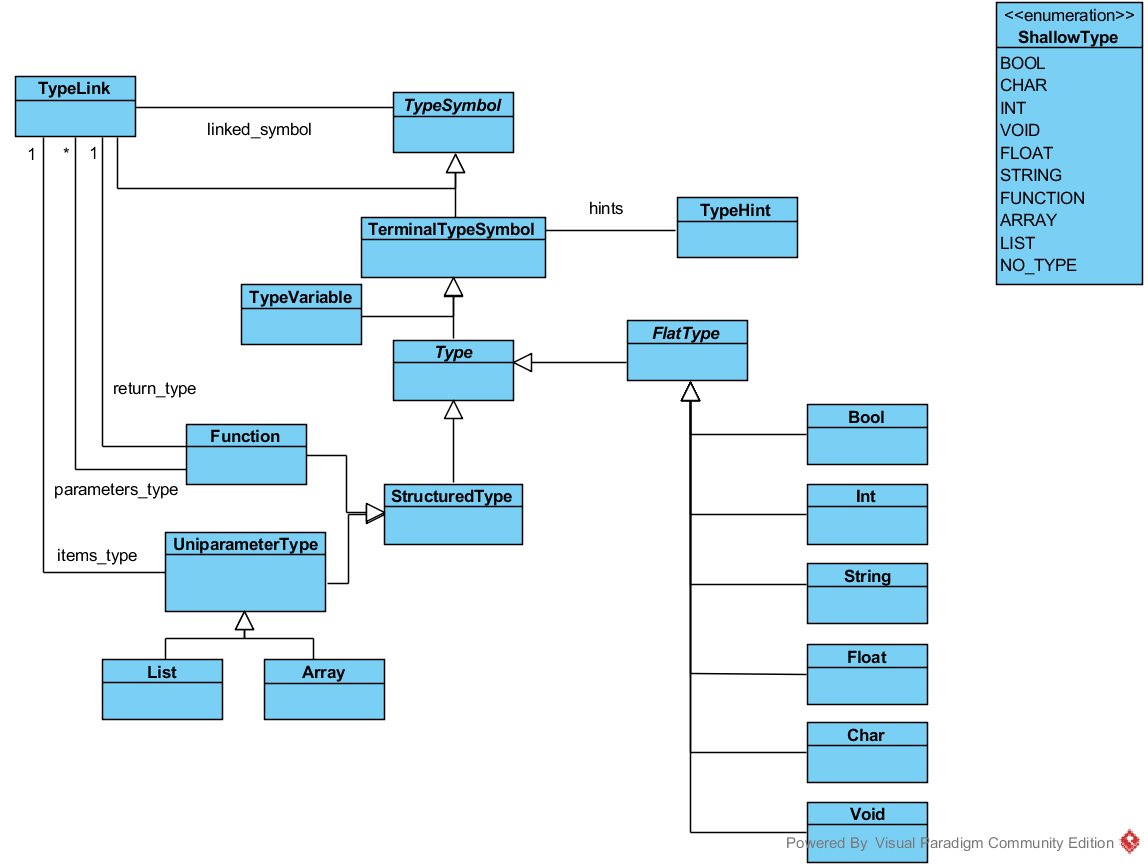
\includegraphics[scale=0.75]{type_symbols.png}
	\caption{Type symbols class diagram}
	\label{fig:}
\end{figure}

\subparagraph{Type symbol table} The type symbol table inherits from an instantiation of the C++ standard hashtable template class, \texttt{std::unordered\_map<std::string,TypeLink>}, and encapsulates the following operations :
\begin{itemize}
	\item unification between two variables
	\item unification between a variable and a flat type
	\item update of the hints of a type variable
	\item creation of new variables
	\item construction of type symbol objects for variables, functions, arrays and lists
	\item construction of a type object for the code generation phase
	\item generation of unique type variable names 
\end{itemize} 
The table stores two kind of variables : the ones bounded to the program's identifiers (so-called \textit{bounded} type variables) and the ones that are not (so-called \textit{pure} type variables). As every variable has to be uniquely identified, the generation of variable names have to be done carefully :
\begin{itemize}
	\item pure variable names are numbers generated with a counter and is therefore collision free as long as the counter does not overflow
	\item as a in a valid program, two identifiers having the same name cannot be declared in the same scope, a unique name for bounded variables can be constructed from these two elements. An additional character, '@' is added between the identifier name and the scope id for the sake of readability. The name of a bounded variable is therefore generated as follows :
	\begin{center}
		\texttt{identifier}@\texttt{scope\_id}
	\end{center}
\end{itemize}
\subparagraph{Syntax-directed type inference} As every other semantic analysis pass, the type inference is implemented with another visitor in \texttt{TypeInferenceVisitor.cpp}. Each node corresponds to a language construct of which the type semantic must be translated in the type symbol table. Moreover, a node can receive from its parent and pass to his children a set of variable (for instance, if an expression is expected to return a value of a given type, the corresponding type variable could be passed from the parent to the expression node). Therefore, designing the type inference for a node results in answering five questions :
\begin{enumerate}
	\item \textbf{Inheritance} : which type variables are inherited from the parent node?
	\item \textbf{Table insertion} : which variables must be created in the type symbol table and with which terminal type symbols have they to be associated?
	\item \textbf{Unification} : which pairs of variables have to be unified ? Does a variable have to be unified with a flat type?
	\item \textbf{Hinting} : has the hints of a variable to be updated ? 
	\item \textbf{Transmission} : which variables must be given to the children nodes?
\end{enumerate} 
As these elements must be defined for every node, the complete list is not detailed here. Nevertheless, three examples are given : the \textit{+} operator, the \textit{if} statement and the function declaration. 
\begin{itemize}
	\item \textbf{Operator +} : this node has two children, the two operands 
	\begin{itemize}
		\item \textit{Inheritance} : $\alpha$ is the type that should be returned by the operation
		\item \textit{Table insertion} : no type variable insertion 
		\item \textit{Unification} : no unification 
		\item \textit{Hinting} : as '\texttt{+}' can only take integer or float operands, we have : $\mathcal{H}_\alpha = \mathcal{H}_\alpha \cap \{\texttt{int}, \texttt{float}\}$
		\item \textit{Transmission} : as the type returned by the addition is the same as the type of the operands $\alpha$ is passed the both of them
	\end{itemize}
	\item \textbf{Statement \textit{if}} : this node has two children, the condition expression and the scope
	\begin{itemize}
		\item \textit{Inheritance} : $\alpha$ is the type that should be returned by a \texttt{nori} statement in the \textit{if} scope
		\item \textit{Table insertion} : $\beta$ is the type returned by the condition expression
		\item \textit{Unification} : as the condition expression must return a boolean value, the following unification must be performed : $unify(\beta, \texttt{bool})$
		\item \textit{Hinting} : no hinting
		\item \textit{Transmission} : $\beta$ is passed to the condition expression node and $\alpha$ to the scope node
	\end{itemize}
	\item \textbf{Function declaration} : \texttt{maki func\_name p$_1$ ... p$_n$ : scope ;;} (for instance defined in the scope 1 and its scope having id 2)
	\begin{itemize}
		\item \textit{Inheritance} : no inheritance
		\item \textit{Table insertion} : \textit{func\_name@1} is the type of the function, \textit{p$_i$@2} is the type of the $i^{th}$ parameter and $\alpha$ is the return type
		\item \textit{Unification} : the function name must be unified with the function type : 
		\[ unify(\textit{func\_name@1}, \textit{p}_1\textit{@2} \hdots \textit{p}_n\textit{@2} \rightarrow \gamma) \]
		\item \textit{Hinting} : each hinted parameter should be hinted. If the hint is a flat type, an unification can be performed instead
		\item \textit{Transmission} : $\gamma$ to the scope node
	\end{itemize}
\end{itemize}
The \textit{almost} complete list of the nodes and their inference actions is given in the \texttt{Inference.pdf} document attached to the submitted archive.
\subparagraph{Error handling} When an error occurs, the unification errors are added to the error handler with a message indicating the type causing the error, and the one that was expected. If an error occurred during type inference, the next stages are bypassed. As said above, a program passing the type inference without error might not be a valid program, nevertheless an explicit check of this possible problem wasn't implemented but will trigger an exception in the intermediate code generation phase.
\subsection{Intermediate code generation}
\subsubsection{Code construction}
\subsection{Optimization and machine code generation}
The last compile phase is implemented using the C standard \texttt{system} function which "\textit{invokes the command processor to execute a command}" (taken from [\ref{enum:system_cmd_proc}]). Through this function, calls to LLVM utilities are done to optimize the intermediate representation and to generate the executable.
\subsubsection{Optimization}
The LLVM optimizer \texttt{opt} command is used. The optimization performed are the following :
\begin{itemize}
	\item \texttt{mem2reg} : try to use registers instead of memory (as our generation puts everything into memory, this pass is very useful)
	\item \texttt{tailcallelim} : try to perform tail call elimination (transform tail call recursive functions into iterative functions)
	\item \texttt{inline} : try to inline functions from callee to caller (bottom-up)
	\item \texttt{constprop} : try to propagates and merges constants intervening in the program
	\item \texttt{dce} : detect and try to get rid of the dead code blocks (sometimes generated by the compiler, or by the optimizer)
\end{itemize}
By default, the compiler doesn't optimize the generated code. The flag \texttt{-t} must be given to enable these optimizations.
\subsubsection{Machine code generation}
The compiler chains the following commands :
\begin{itemize}
	\item \texttt{clang} : to generate, from source, the LLVM code of the runtime libraries (\texttt{.c} $\rightarrow$ \texttt{.ll})
	\item \texttt{llvm-as} : to compile human readable LLVM to bitcode assembler (\texttt{.ll} $\rightarrow$ \texttt{.bc})
	\item \texttt{llc} : to compile bitcode assembler to machine assembler (\texttt{.bc} $\rightarrow$ \texttt{.s})
	\item \texttt{gcc} : to generate the executable from the \texttt{.s} files
\end{itemize}
The commands \texttt{clang}, \texttt{llvm-as} and \texttt{llc} are extracted from the LLVM \texttt{3.5} bundle and the version of \texttt{gcc} is \texttt{4.8.2}. Yet, nothing fuzzy is done with these commands and using a more recent version should also work (even with older versions for the LLVM commands).
To clean remove the useless generated files, the unix commands \texttt{mv} and \texttt{rm} are also used.
\section{Runtime}
\label{sec:runtime}
Initially, the runtime was supposed to provide support for :
\begin{itemize}
	\item \textbf{memory management} for arrays and lists (i.e. a garbage collector)
	\item \textbf{closures} : to be able to capture variables in functions, a runtime data structure is required to keep a mapping between variables and their addresses
	\item \textbf{basic functionalities} : IO operations and data structure handling
\end{itemize}
The \textit{closures} functionality was dropped due to a lack of time but the others were successfully implemented. Three runtime libraries were implemented :
\begin{itemize}
	\item \texttt{array\_runtime.h} : interface to the array management runtime  
	\item \texttt{list\_runtime.h} : interface to the list management runtime
	\item \texttt{support.h} : interface providing basic operations such as IO (print)
\end{itemize}
The list and array runtimes are implemented using the same principle. A object of type \texttt{struct array\_table} (reps. \texttt{struct list\_table}) contains all the allocated arrays (resp. lists) which are identified by a unique number. A set of operations are then provided by the interfaces to interact with an array (resp. a list) given the table object and the array id (resp. list id). Some of these operations are exposed to the \textit{Sushi++} programmer while others (such as reference counting, allocation,...) aren't.
\\
The memory is therefore handled by reference counting through the functions \texttt{array\_add\_reference} and \texttt{array\_rm\_reference} (resp. \texttt{list\_add\_reference} and \texttt{list\_rm\_reference}) that must be called in the LLVM generated program to signal that a data structure is referenced by a new variable or it is not referenced anymore. When the counter drops to 0, the object is automatically freed.
\\
The underlying implementation of the \texttt{struct array\_table} (resp. \texttt{struct list\_table}), stores the arrays (resp. lists) in a linked list which is not optimal but discussed in the Section \
\section{Limitations and possible improvements}
\subsection{Lexical and syntax analysis}
\label{ssec:flaws_syntax}
As mentioned in the Section \ref{ssec:lex_synt}, the semantic type of the node is \texttt{void*}. This choice was done juste before the first deadline because using pointers to actual node objects was triggering weird compile-errors and we weren't able to solve them in another way than using the type \texttt{void*}. This is unfortunate because it makes the code longer and less readable due to type conversion. When we (re)tried, later on, to use actual nodes objects, it seemed to work but we decided not to do it because it would take too much time. An improvement in terms of readability would be to use proper types then.
\\
As the error reporting of \texttt{bison} is used, we rely on the underlying implementation. Therefore, even though we tried to display as much errors as possible, the error reporting is quite erratic. Sometimes, one error will be displayed even if the program contains more, sometimes it will display all of them. Moreover, we discovered a segmentation fault in the \textit{bison} implementation for some erroneous program (which we didn't have time to debug). Adding some \texttt{error} rules in the parser would allow a more fine-grained error reporting. \\
Another problem is the column counting which is buggy. While the line count is accurate, the lexer fails at counting the starting and ending column of a token. Therefore, all the error reports throughout the execution of the program fails at given the correct column of an error. This is why we have disable a interesting feature of the error handler which consisted in displaying the program line triggering an error.
\subsection{Scope and termination checking}
\subsection{Type Inference}
The type inference is quite satisfying even if it can sometimes fail for programs that aren't expressive enough. Few improvements can still be performed :
\begin{itemize}
	\item adding information in the \textbf{type error messages} : for the moment, the messages only report the location where the type checking fails, it would be interesting to know where was generated the constraint that led to the error
	\item adding a \textbf{check for unresolved types} : then the user could be noticed about the lack of expressiveness of its program with precise information
\end{itemize} 
\subsection{Optimization and machine code generation}
As the optimization is performed by another application, improving it is impossible. Nevertheless, some others optimizations passes could be applied (as the \texttt{opt} command provides a lot more than 5 optimization passes). \\
As far as the machine code generation is concern, two problems arise :
\begin{itemize}
	\item \textbf{system dependence} : as the compiler uses unix commands, it could only be used on unix-based operating systems which is configured so that \texttt{gcc} and LLVM commands can be used. Removing these dependencies would allow to port the application on other platform.
	\item \textbf{file dependence and generation} : on the one hand, the compiler needs the implementation files of the runtime to be able to execute machine code generation and therefore couldn't be used as a standalone executable. On the other hand, the compiler generates a lot of files without checking their names. Therefore, finding a way to embed the runtime files into the executable would allow an easier use of the compiler and a system that checks existing file names would prevent troubles caused by collisions.
\end{itemize}
\subsection{Runtime}
\label{ssec:flaws_runtime}
As said in the Section \ref{sec:runtime}, the internal data structure (called \textit{table}) used to store arrays and lists is itself a list. Therefore, accessing an element (list or array) has the a complexity $\mathcal{O}(n)$ where $n$ is the number of objects in the table. Moreover, every function of the interface has to access a particular object in the table before performing operations, this resulting in a search at every function call. This is of course extremely inefficient. The reason why the list implementation was chosen is mainly lack of time. As a simply linked list is easy to implement, we could focus on the code generation instead. A major improvement would then be the reimplementation of the tables with an adequate data structure such as an ordered vector (ordered on the array/list id), a tree or a hashtable. Nevertheless, as implementation details don't leak through the interface, this can be done without changing the code generation.
\\
Also, initially, we wanted to implement closures but we dropped this feature due to lack of time. A improvement in the usability of the language would be the implementation of such a mechanisms. This would include the implementation of another runtime module for handling it (and some parts of the compiler would also have to be modified).
\appendix
\section{Sources}
\begin{enumerate}
	\item \textbf{Lexical and syntax analysis} : 
	\begin{enumerate}
		\item\label{enum:flex_ref} Flex documentation, "\textit{Lexical Analysis With Flex}", \texttt{http://goo.gl/wIJglV}
		\item\label{enum:bison_ref} Charles Donnely, Richard Stallman, "\textit{Bison, Using the Yacc-compatible Parser Generator}", \texttt{http://goo.gl/rp2kpM} 
	\end{enumerate}
	\item \textbf{Type inference} : 
	\begin{enumerate}
		\item\label{enum:inference_unification} Paul N. Hilfinger, "\textit{Lecture \#22: Type Inference and Unification}", \texttt{https://goo.gl/RR8Eme}, UC Berekeley, course \textit{CS164} : Programming Languages and Compilers.
		\item\label{enum:inference_photon} Cyril Soldani, "\textit{Monomorphic type inference}", \texttt{http://goo.gl/Kveyvf}
	\end{enumerate}
	\item \textbf{Optimization and machine code generation}
	\begin{enumerate}
		\item\label{enum:system_cmd_proc} CPlusPlus.com, "\textit{\texttt{system} - C++ reference}", \texttt{http://goo.gl/XkM9rr}
		\item\label{enum:opt_passes} LLVM documentation, "\textit{LLVM’s Analysis and Transform Passes}", \texttt{http://goo.gl/P8kyxX}
	\end{enumerate}
\end{enumerate}
\end{document}